\documentclass[12pt, a4paper, oneside]{article}
\usepackage[utf8]{vietnam}
\usepackage[utf8]{inputenc}
\usepackage[top = 2.5cm, bottom = 2.5cm, left = 1.5cm, right = 1cm]{geometry}
\usepackage{amsmath,amsfonts,amssymb}
\usepackage{indentfirst,enumitem}
\usepackage{graphicx}
\usepackage{multicol}
\usepackage{multirow}
\usepackage{setspace}
\usepackage{hyperref}
\usepackage{listings}
\usepackage{tabularx}
\usepackage{hyperref}
\usepackage{xcolor}
\usepackage{scrextend}
\usepackage{comment}
\usepackage{soul}
\usepackage{tipa}
\usepackage{subcaption}
\usepackage{caption}
\usepackage{booktabs}
\usepackage{array}
\usepackage{fancyhdr}
\usepackage{algorithm2e}
\usepackage{float}
\usepackage[most]{tcolorbox}
\usepackage{pdfpages}
\usepackage{import}
\graphicspath{ {figures/} }

\usepackage{float}
\usepackage{tikz}
\usetikzlibrary{calc, positioning, shapes.geometric}
\usetikzlibrary{circuits.logic.US, circuits.logic.IEC}

\captionsetup[figure]{labelfont=bf, textfont=it, font=small}

\hypersetup{
    colorlinks=true,
    linkcolor=blue,
    filecolor=magenta,      
    urlcolor=blue,
    pdftitle={DTUD},
}

%\changefontsizes{13pt}
\renewcommand\thesection{\arabic{section}.}
\renewcommand\thesubsection{\arabic{section}.\arabic{subsection}}

\pagestyle{fancy}
\fancyhead[r]{\textit{GVHD: Nguyễn Trung Hiếu}}
%\fancyhead[c]{\bfseries DSP}
\fancyhead[l]{\textit{Điện tử Ứng dụng}}
\renewcommand{\headrulewidth}{0.2pt}
\setlength{\headheight}{10pt}


\def\mathrlap{\mathpalette\mathrlapinternal} 
\def\mathclap{\mathpalette\mathclapinternal}
\def\mathllapinternal#1#2{\llap{$\mathsurround=0pt#1{#2}$}}
\def\mathrlapinternal#1#2{\rlap{$\mathsurround=0pt#1{#2}$}}

%CHÈN ẢNH
\usepackage{pgfplots}
\pgfplotsset{compat=1.15}
\usepackage{mathrsfs}
\usetikzlibrary{arrows}
\usetikzlibrary[patterns]

%New colors defined below
\definecolor{codegreen}{rgb}{0,0.6,0}
\definecolor{codegray}{rgb}{0.5,0.5,0.5}
\definecolor{codepurple}{rgb}{0.58,0,0.82}
\definecolor{backcolour}{rgb}{0.95,0.95,0.92}

\begin{document}
% Định nghĩa macro vẽ ký hiệu tam giác cho chân Clock
\def\clktriangle#1#2{
    \draw (#1, #2) ++(0, 0.15) -- ++(0.2, -0.15) -- ++(-0.2, -0.15);
}
\begin{titlepage}
%\SetWatermarkText{\includegraphics[width = 0.97\paperwidth,
%height = 0.97\paperheight]{bia.png}}
%\SetWatermarkAngle{0} 
%\SetWatermarkText{\includegraphics[scale=1]{hust.png}}
%\SetWatermarkAngle{0} 
\begin{tikzpicture}[remember picture,overlay,inner sep=0,outer sep=0]
     \draw[blue!70!black,line width=4pt] ([xshift=-1.5cm,yshift=-2cm]current page.north east) coordinate (A)--([xshift=1.5cm,yshift=-2cm]current page.north west) coordinate(B)--([xshift=1.5cm,yshift=2cm]current page.south west) coordinate (C)--([xshift=-1.5cm,yshift=2cm]current page.south east) coordinate(D)--cycle;

     \draw ([yshift=0.5cm,xshift=-0.5cm]A)-- ([yshift=0.5cm,xshift=0.5cm]B)--
     ([yshift=-0.5cm,xshift=0.5cm]B) --([yshift=-0.5cm,xshift=-0.5cm]B)--([yshift=0.5cm,xshift=-0.5cm]C)--([yshift=0.5cm,xshift=0.5cm]C)--([yshift=-0.5cm,xshift=0.5cm]C)-- ([yshift=-0.5cm,xshift=-0.5cm]D)--([yshift=0.5cm,xshift=-0.5cm]D)--([yshift=0.5cm,xshift=0.5cm]D)--([yshift=-0.5cm,xshift=0.5cm]A)--([yshift=-0.5cm,xshift=-0.5cm]A)--([yshift=0.5cm,xshift=-0.5cm]A);


     \draw ([yshift=-0.3cm,xshift=0.3cm]A)-- ([yshift=-0.3cm,xshift=-0.3cm]B)--
     ([yshift=0.3cm,xshift=-0.3cm]B) --([yshift=0.3cm,xshift=0.3cm]B)--([yshift=-0.3cm,xshift=0.3cm]C)--([yshift=-0.3cm,xshift=-0.3cm]C)--([yshift=0.3cm,xshift=-0.3cm]C)-- ([yshift=0.3cm,xshift=0.3cm]D)--([yshift=-0.3cm,xshift=0.3cm]D)--([yshift=-0.3cm,xshift=-0.3cm]D)--([yshift=0.3cm,xshift=-0.3cm]A)--([yshift=0.3cm,xshift=0.3cm]A)--([yshift=-0.3cm,xshift=0.3cm]A);

   \end{tikzpicture}
\begin{center}
    \vspace{7pt}
        \textbf{ĐẠI HỌC QUỐC GIA THÀNH PHỐ HỒ CHÍ MINH}
    
    \vspace{7pt}
    \textbf{TRƯỜNG ĐẠI HỌC BÁCH KHOA}
    
    \vspace{7pt}
    \textbf{KHOA ĐIỆN - ĐIỆN TỬ}
\end{center}
\vspace{10pt}
\begin{center}
    
\includegraphics[scale=0.3]{2_img/HCMUT.png}
    \vspace{10pt}
\end{center}

\begin{center}
    \fontsize{18pt}{17pt}\selectfont 
    \textbf{BÁO CÁO BÀI TẬP LỚN SỐ 1}

    \textbf{MÔN: ĐIỆN TỬ ỨNG DỤNG}
\end{center}
\begin{center}
    \fontsize{15pt}{17pt}\selectfont 
    \textbf{\textrm{Đề 3: Thiết kế mạch đo nhiệt độ sử dụng Thermistor.}}
\end{center}

\begin{center}
    \vspace{15pt}
    \textbf{Lớp: L01 - NHÓM: 7}
    
    \textbf{GVHD: ThS. Nguyễn Trung Hiếu}
\end{center}

\vspace{10pt}

\begin{table}[h!]
\centering
\begin{tabular}{|c|c|c|}
\hline
\textbf{MSSV} & \textbf{Họ và tên} & \textbf{Tỉ lệ phân công} \\ \hline
2210570 & Hoàng Anh Dũng & 100\% \\ \hline
2311267 & Vũ Nhật Huy & 100\% \\ \hline
2412954 & Phan Văn Quyết & 100\% \\ \hline
\end{tabular}
\end{table}
\vfill
\centerline{\bf Thành phố Hồ Chí Minh, tháng 11 năm 2026}

\vspace{1cm}
\end{titlepage}
\newpage
\tableofcontents
\newpage
\listoffigures
\newpage
\section*{ĐỀ TÀI 3}
Thiết kế mạch đo nhiệt độ sử dụng Thermistor. Mạch có tầm đo 20 - 80°C, độ phân giải 0.1°C, ngõ ra là dòng điện tương ứng từ 4-20mA (nối đất):
\begin{itemize}
    \item[a.] Lựa chọn và mô phỏng Thermistor 2 dây (có điện trở dây dẫn là $10 \varOmega$).
    \item[b.] Lựa chọn điện trở song song để tuyến tính hóa.
    \item[c.] Lựa chọn OPAMP sử dụng, mô phỏng OPAMP theo datasheet.
    \item[d.] Đảm bảo sai số (giữa giá trị lý thuyết và thực tế đo qua mạch) $\pm 5\%$.
    \item[e.] Thiết kế mạch đọc dòng điện và cho ngõ ra ADC. Tiến hành lựa chọn ADC (số bit, nguồn). Mô phỏng mạch đọc và kiểm chứng.
\end{itemize}

\newpage
\section{Lựa chọn và mô phỏng Thermistor 2 dây (có điện trở dây dẫn là $10 \varOmega$).}
\subsection{Lựa chọn}
Với Thermistor 2 dây, với mỗi dây có điện trở dây dẫn là $10 \varOmega$, với tầm đo là $20^o C \to 80^o C$ và span là $60^o C$. Nhóm em quyết định chọn con Thermistor NTC là \href{https://www.vishay.com/en/product/29049/}{NTCLE100E3} với các thông số tổng quan được thể hiện qua hình \ref{fig:1}:
\begin{figure}[H]
    \centering
    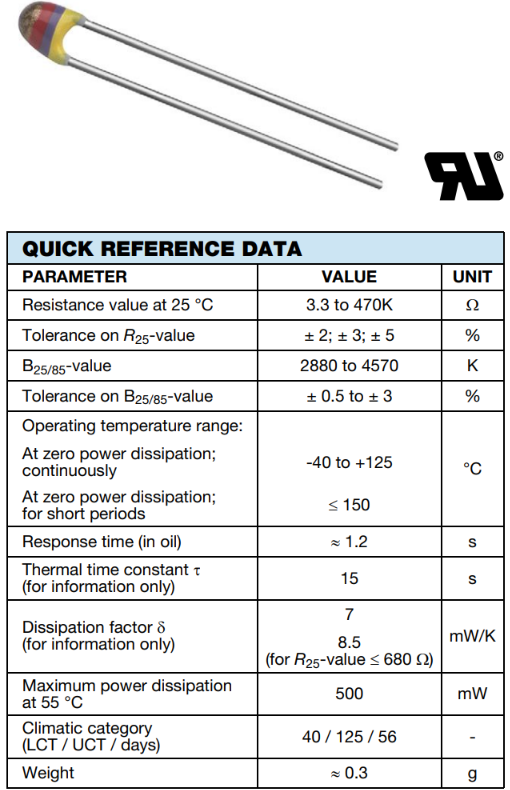
\includegraphics[width=0.65\linewidth]{2_img/1.png}
    \caption{Chi tiết thông số linh kiện NTCLE100E3.}
    \label{fig:1}
\end{figure}
\newpage
\subsection{Mô phỏng}

%%%%%%%%%%%%%%%%%%%%%%%%%%%%%%%%%%%%%%%%%%%%
\section{Lựa chọn điện trở song song để tuyến tính hóa.}
%%%%%%%%%%%%%%%%%%%%%%%%%%%%%%%%%%%%%%%%%%%%
\section[Lựa chọn OPAMP sử dụng, mô phỏng OPAMP theo datasheet.]{Lựa chọn OPAMP sử dụng, mô phỏng OPAMP theo\\ datasheet.}




%%%%%%%%%%%%%%%%%%%%%%%%%%%%%%%%%%%%%%%%%%%%
\section{Đảm bảo sai số (giữa giá trị lý thuyết và thực tế đo qua mạch) $\pm 5\%$.}
%%%%%%%%%%%%%%%%%%%%%%%%%%%%%%%%%%%%%%%%%%%%
\section{Thiết kế mạch đọc dòng điện và cho ngõ ra ADC. Tiến hành lựa chọn ADC (số bit, nguồn). Mô phỏng mạch đọc và kiểm chứng.}
%%%%%%%%%%%%%%%%%%%%%%%%%%%%%%%%%%%%%%%%%%%%

\end{document}